\documentclass[10pt]{article}
\usepackage{tikz}
\usepackage[margin=0cm]{geometry}
\pagestyle{empty}

\begin{document}

\vspace*{\fill}
\begin{center}
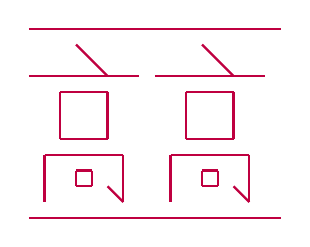
\begin{tikzpicture}[x=0.2cm, y=-0.2cm, thick, purple]
% North to South lines
    \draw (1,8) -- (1,11);
    \draw (2,4) -- (2,7);
    \draw (3,9) -- (3,10);
    \draw (4,9) -- (4,10);
    \draw (5,4) -- (5,7);
    \draw (6,8) -- (6,11);
    \draw (9,8) -- (9,11);
    \draw (10,4) -- (10,7);
    \draw (11,9) -- (11,10);
    \draw (12,9) -- (12,10);
    \draw (13,4) -- (13,7);
    \draw (14,8) -- (14,11);
% North-West to South-East lines
    \draw (3,1) -- (5,3);
    \draw (11,1) -- (13,3);
    \draw (5,10) -- (6,11);
    \draw (13,10) -- (14,11);
% West to East lines
    \draw (0,0) -- (16,0);
    \draw (0,3) -- (7,3);
    \draw (8,3) -- (15,3);
    \draw (2,4) -- (5,4);
    \draw (10,4) -- (13,4);
    \draw (2,7) -- (5,7);
    \draw (10,7) -- (13,7);
    \draw (1,8) -- (6,8);
    \draw (9,8) -- (14,8);
    \draw (3,9) -- (4,9);
    \draw (11,9) -- (12,9);
    \draw (3,10) -- (4,10);
    \draw (11,10) -- (12,10);
    \draw (0,12) -- (16,12);
% South-West to North-East lines
\end{tikzpicture}
\end{center}
\vspace*{\fill}

\end{document}
